% Skipping a bunch of chapters
\chapter{Line Segment Tracking}

\section{The HL-LHC computing challenge}

\begin{figure}[htb]
  \centering
  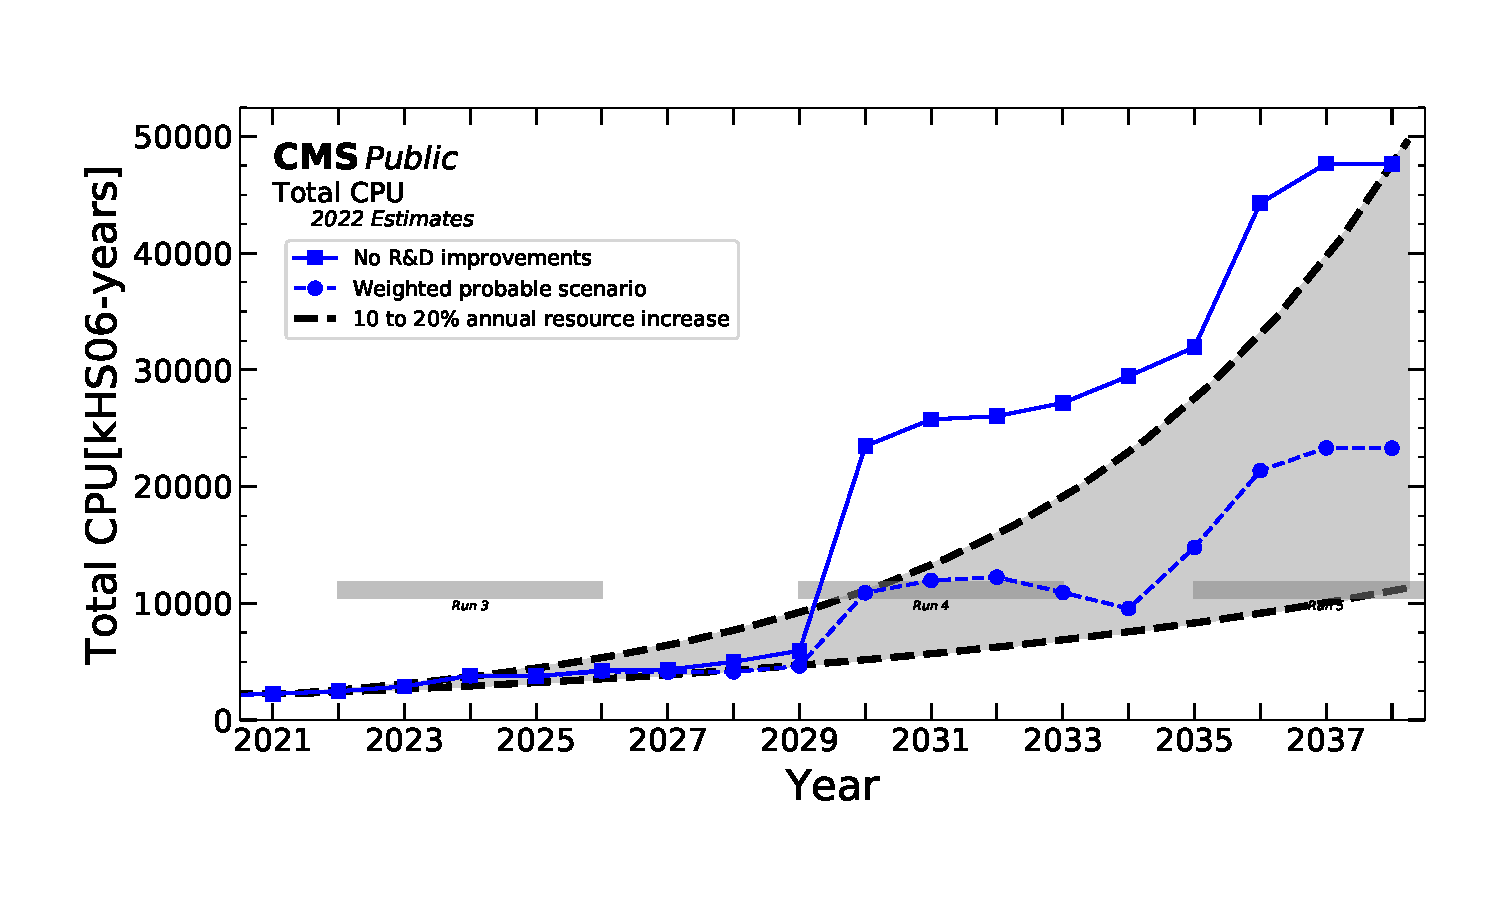
\includegraphics[width=.9\textwidth]{fig/lst/cpu_cms2022.pdf}
  \caption{Lorem ipsum~\cite{CMSComputingReport2022}.}
  \label{fig:cpu_projections}
\end{figure}

\subsection{Track reconstruction}

\begin{figure}[!htb]
  \centering
  \subfloat{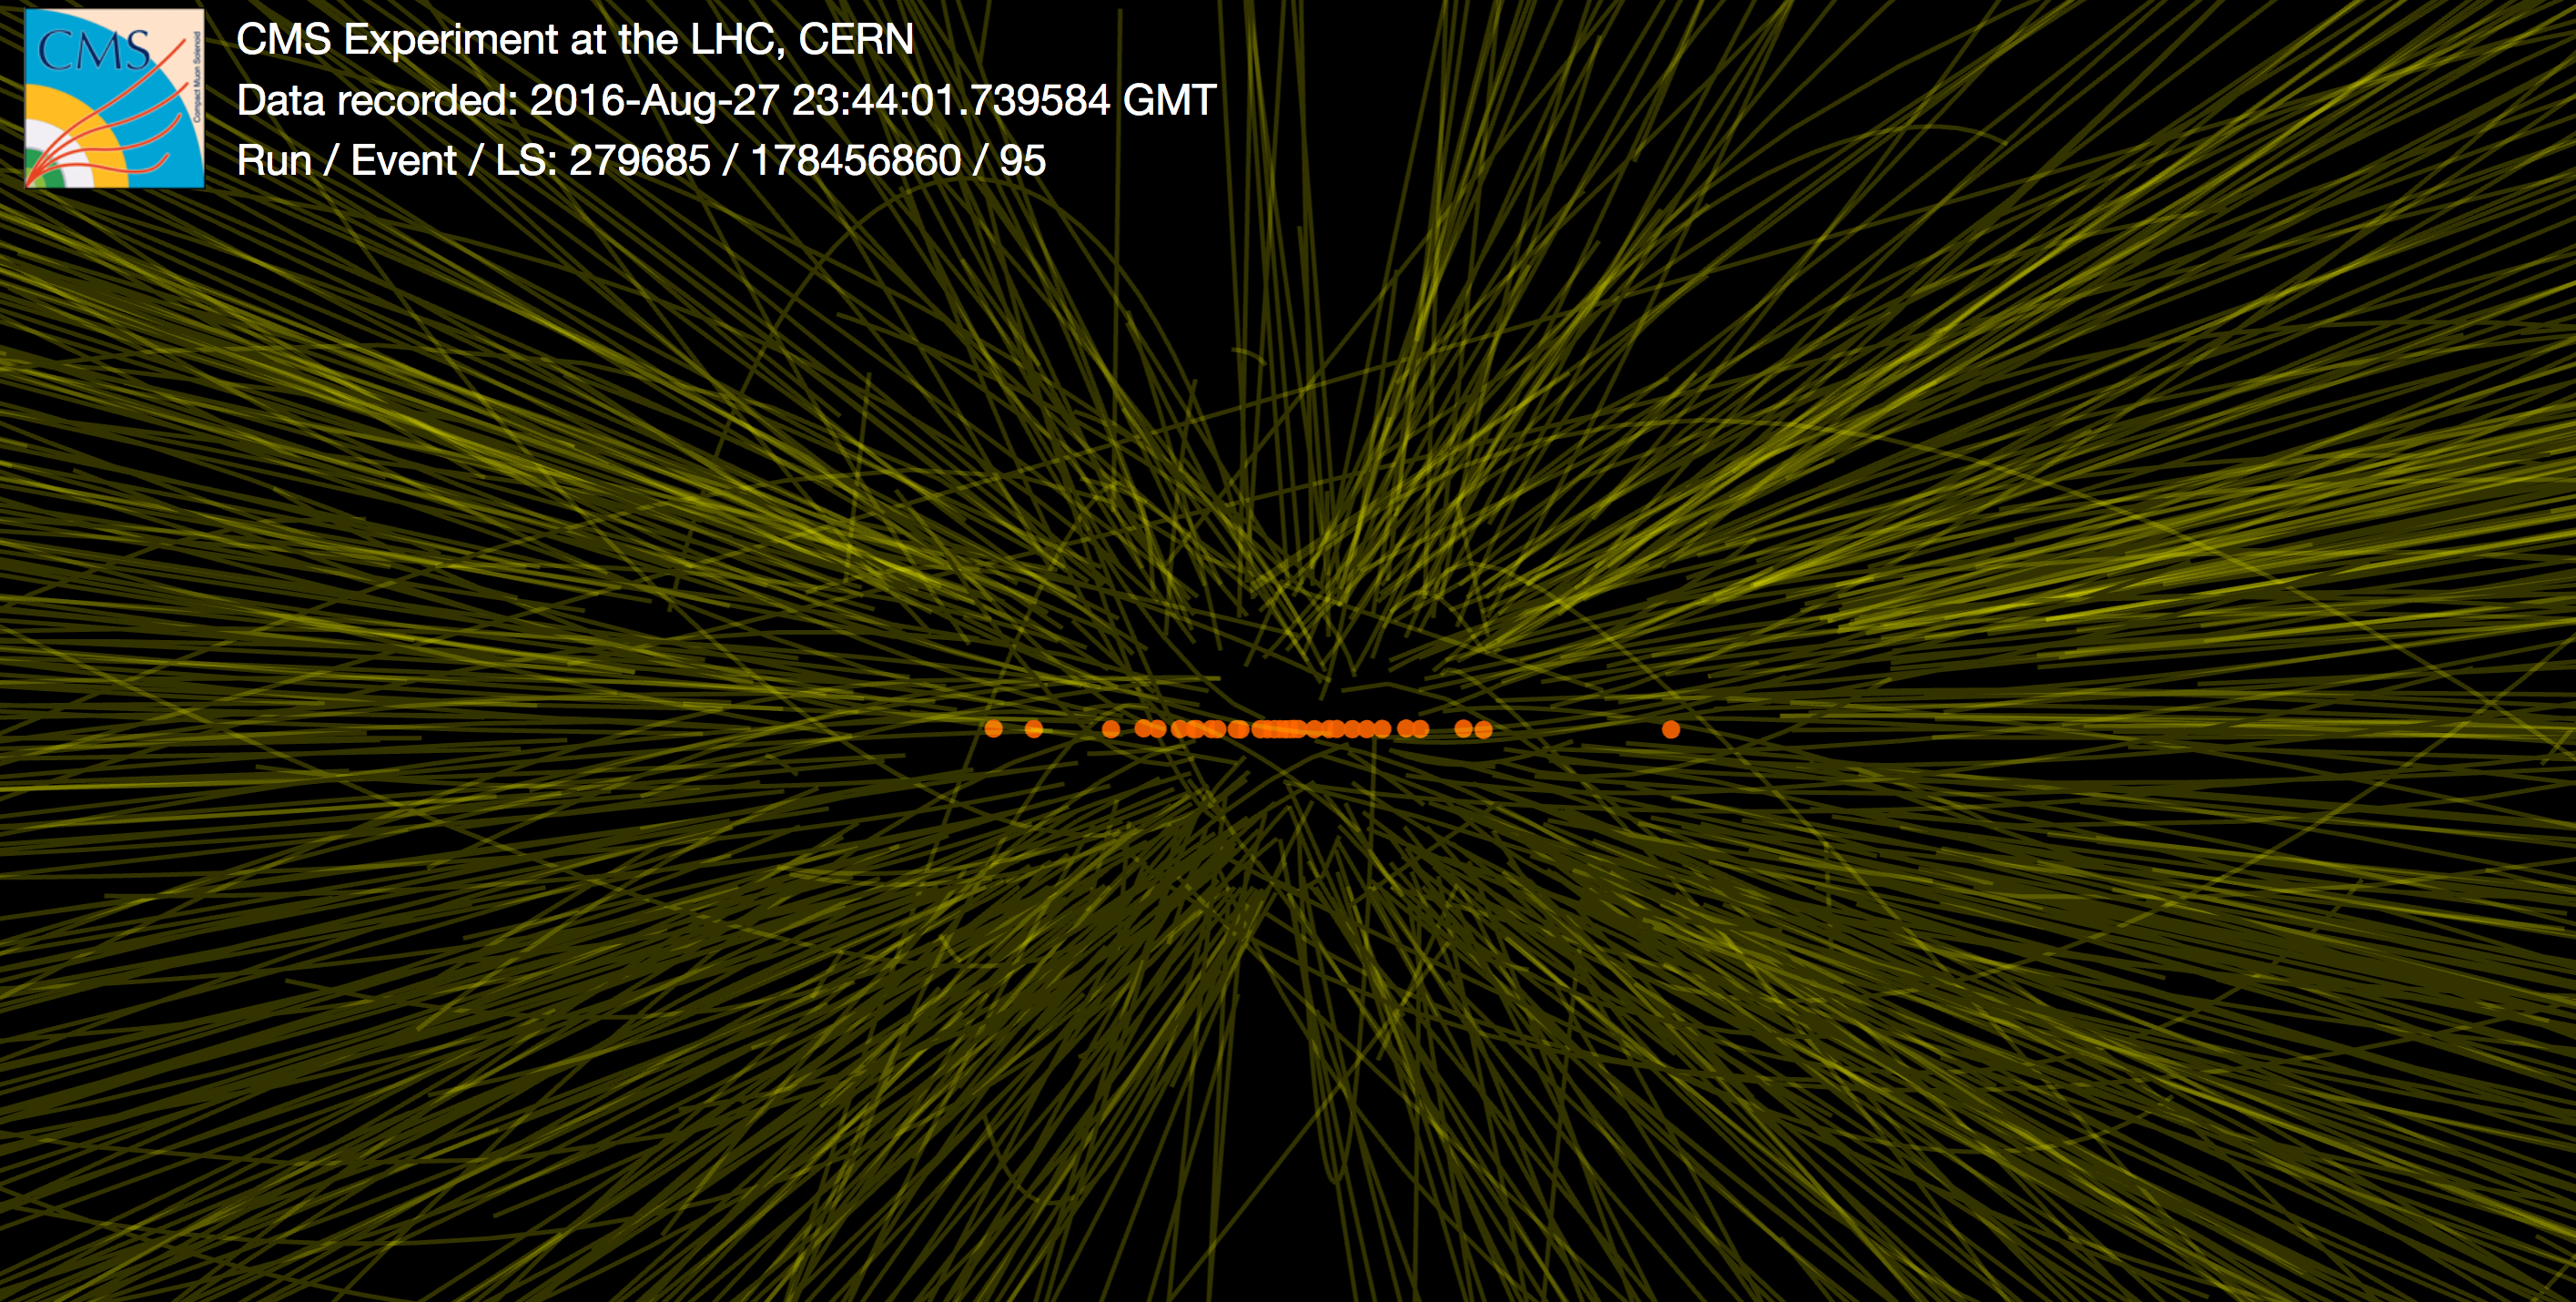
\includegraphics[width=0.45\linewidth]{fig/lst/high_PU_30vtx_side.png}}
  \qquad
  \subfloat{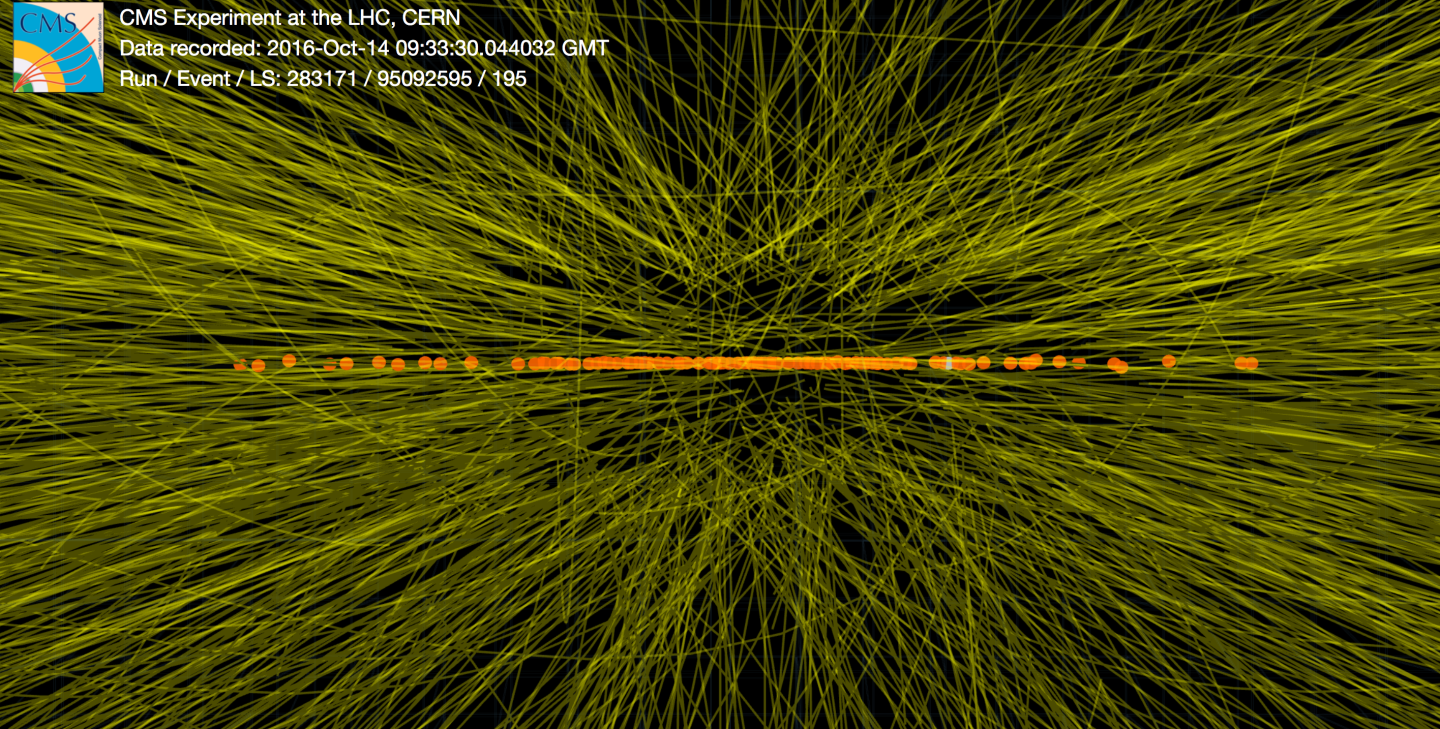
\includegraphics[width=0.45\linewidth]{fig/lst/high_PU_130vtx.png}}
  \caption{
      A collision event with standard pile-up (left) recorded at CMS in 2016 is shown next to an event with HL-LHC-like pile-up (right) recorded at CMS in the same year~\cite{NormalPU2016, HighPU2016}.
      The dots are proton-proton collisions and the thin lines are the reconstructed particle tracks.
  }
  \label{fig:pileup}
\end{figure}

\section{The line segment tracking algorithm}

\begin{figure}[!htb]
  \centering
  \subfloat{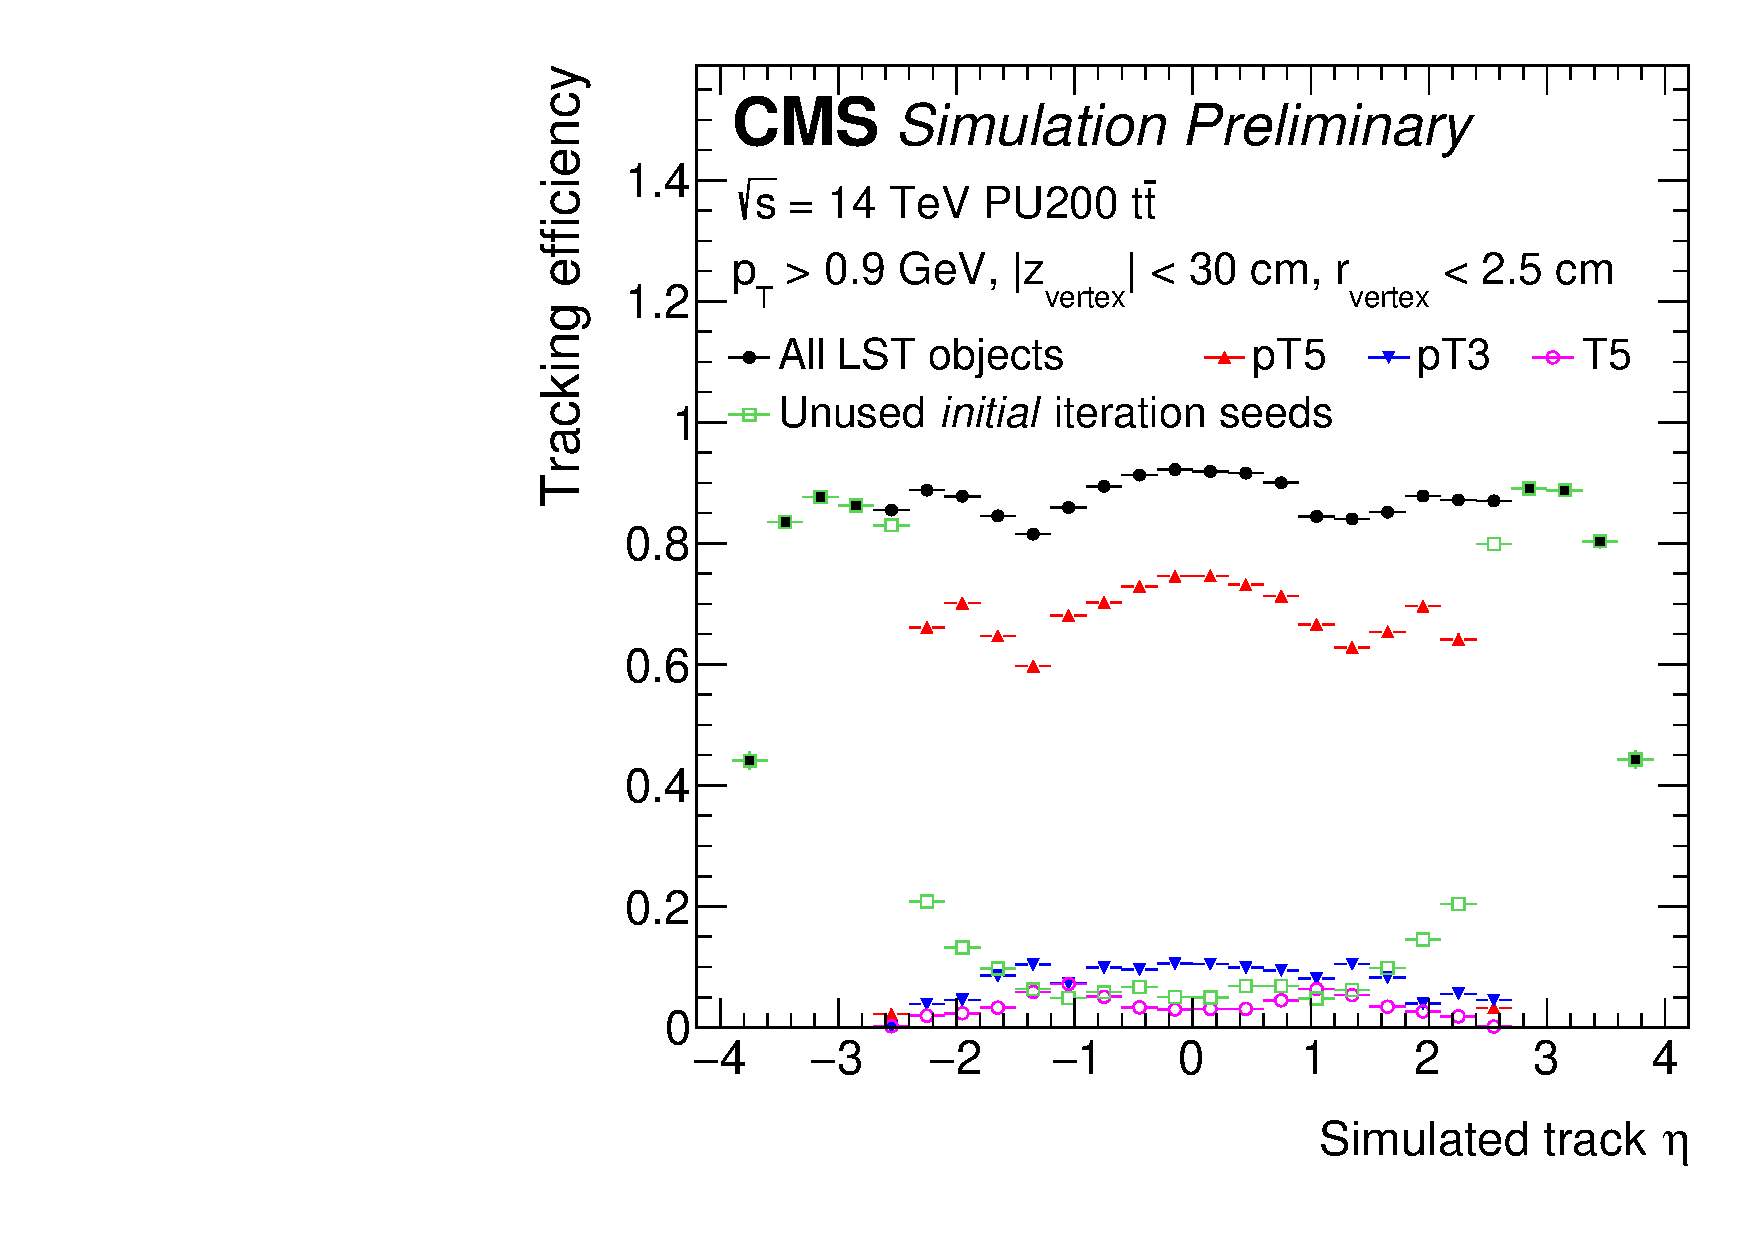
\includegraphics[width=0.45\linewidth]{fig/lst/standalone_Master_eff_etacourse.pdf}}
  \qquad
  \subfloat{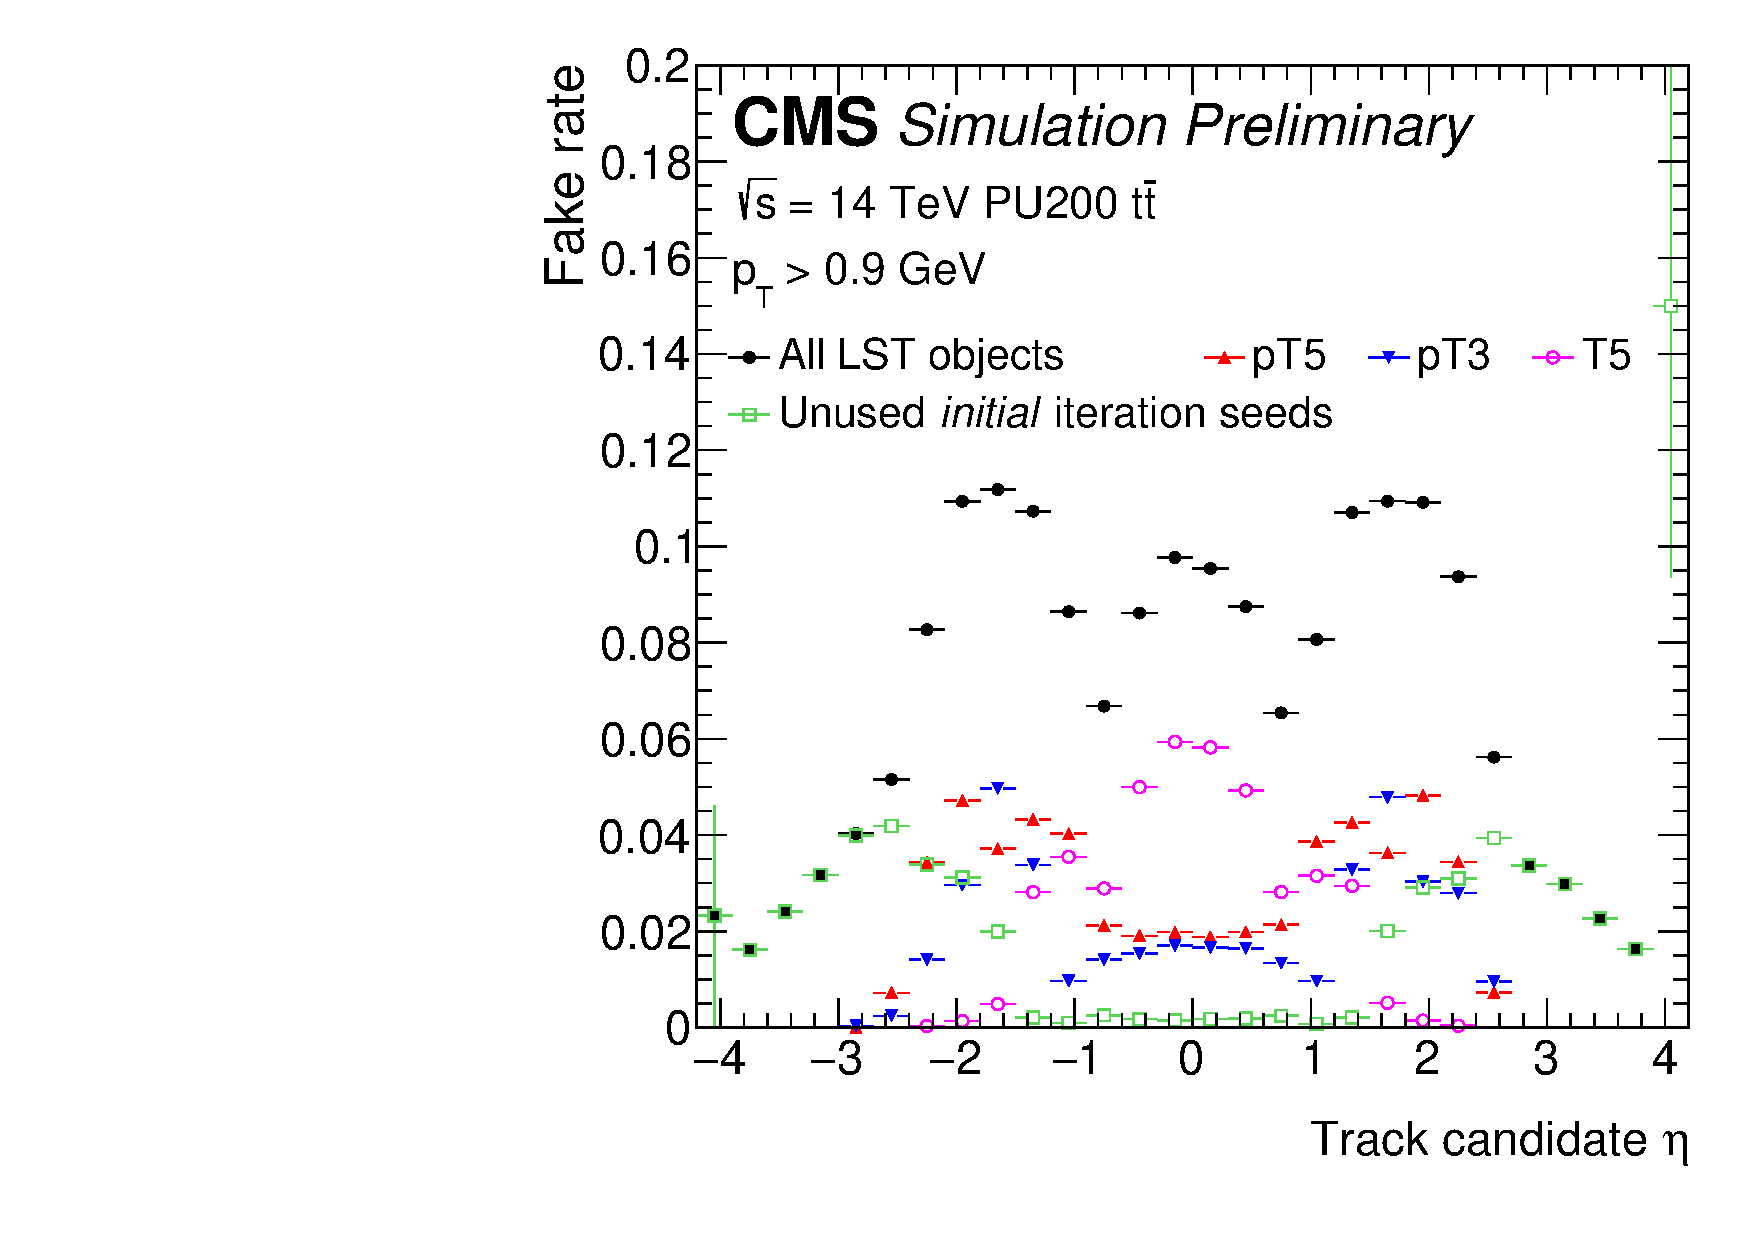
\includegraphics[width=0.45\linewidth]{fig/lst/standalone_Master_fr_etacourse.pdf}}
  \caption{
      The LST track-finding efficiency (left) and fake rate (right) are plotted as a function of the pseudorapidity $\eta$ of the simulated track and track candidate respectively.
      For both plots, five histograms are overlayed: all track candidates (black), pT5s (red), pT3s (blue), T5s (magenta), and pLSs that are not used in a pT5 or pT3 (green).
      On the left, it can be seen that T5s comprise the majority of the LST track-finding efficiency, either as pT5s or T5s.
      On the right, it can also be seen that the T5s make up the bulk of the LST fake rate in the barrel region.
  }
  \label{fig:lst_performance}
\end{figure}

\section{Improving LST with machine learning}

\begin{figure}[!htb]
  \centering
  \subfloat[]{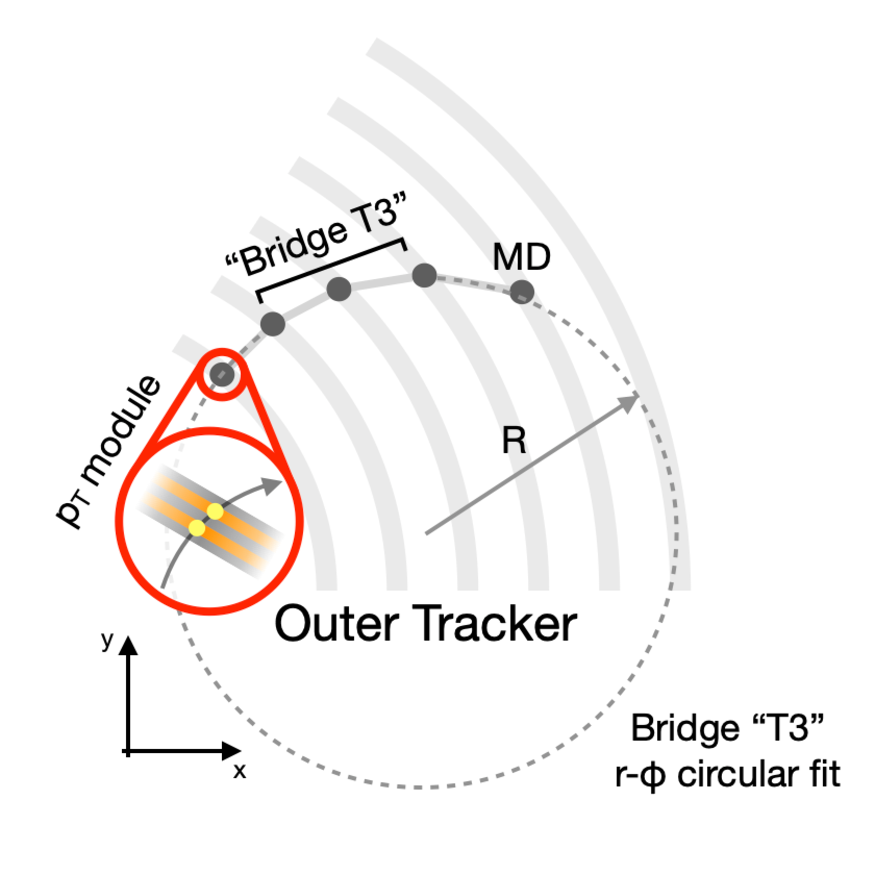
\includegraphics[width=0.35\linewidth]{fig/lst/T5_anatomy.pdf}\label{fig:t5_anatomy}}
  \qquad
  \subfloat[]{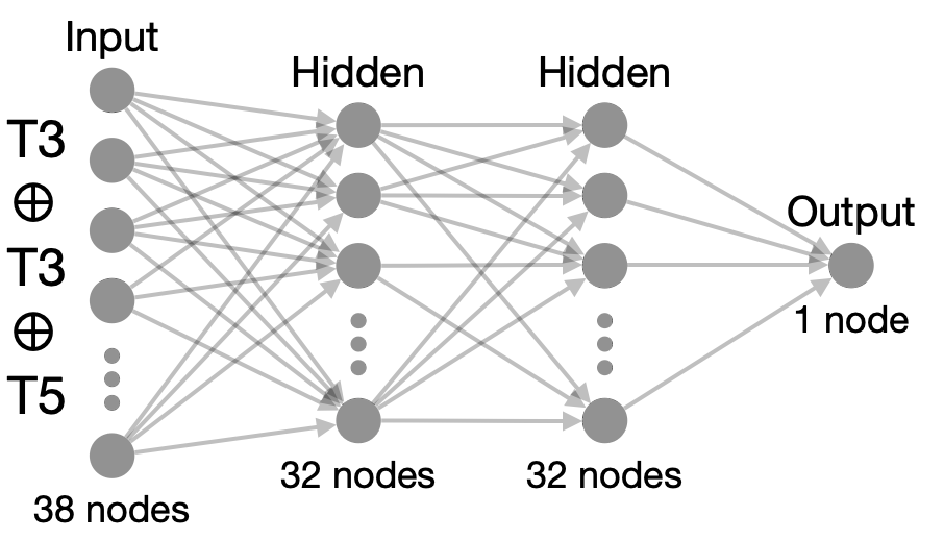
\includegraphics[width=0.55\linewidth]{fig/lst/T5_DNN_architecture.pdf}\label{fig:t5dnn_arch}}
  \caption{
      Lorem ipsum.
  }
\end{figure}

\begin{figure}[!htb]
  \centering
  \subfloat[]{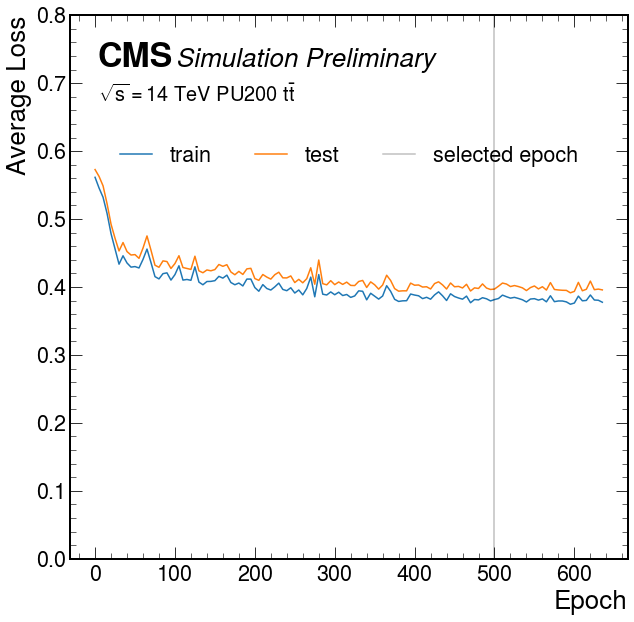
\includegraphics[width=0.45\linewidth]{fig/lst/main_history.png}\label{fig:t5dnn_history}}
  \qquad
  \subfloat[]{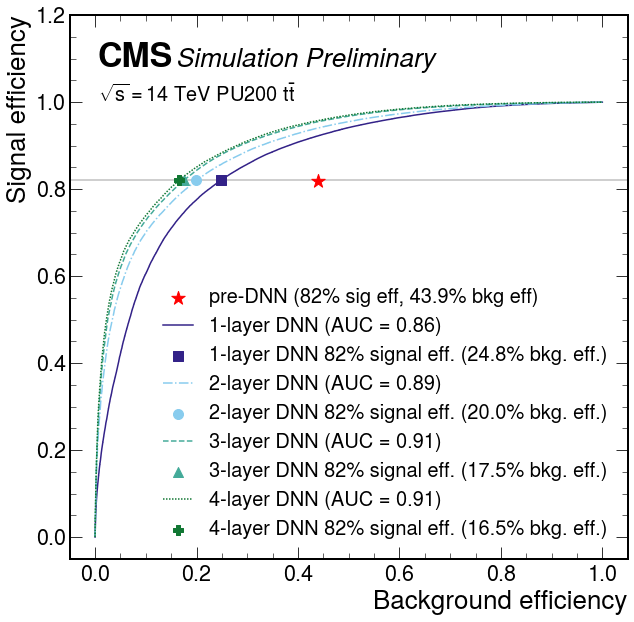
\includegraphics[width=0.45\linewidth]{fig/lst/roc.png}\label{fig:t5dnn_roc}}
  \caption{
      The average loss after each epoch is plotted (a) next to the Receiver Operating Characteristic (ROC) curves for the model after epoch 500 (b). 
      For the ROC curve, the signal efficiency is plotted on the y-axis, while the background efficiency, or fake rate, is plotted on the x-axis. 
  }
\end{figure}

\begin{figure}[!htb]
  \centering
  \subfloat{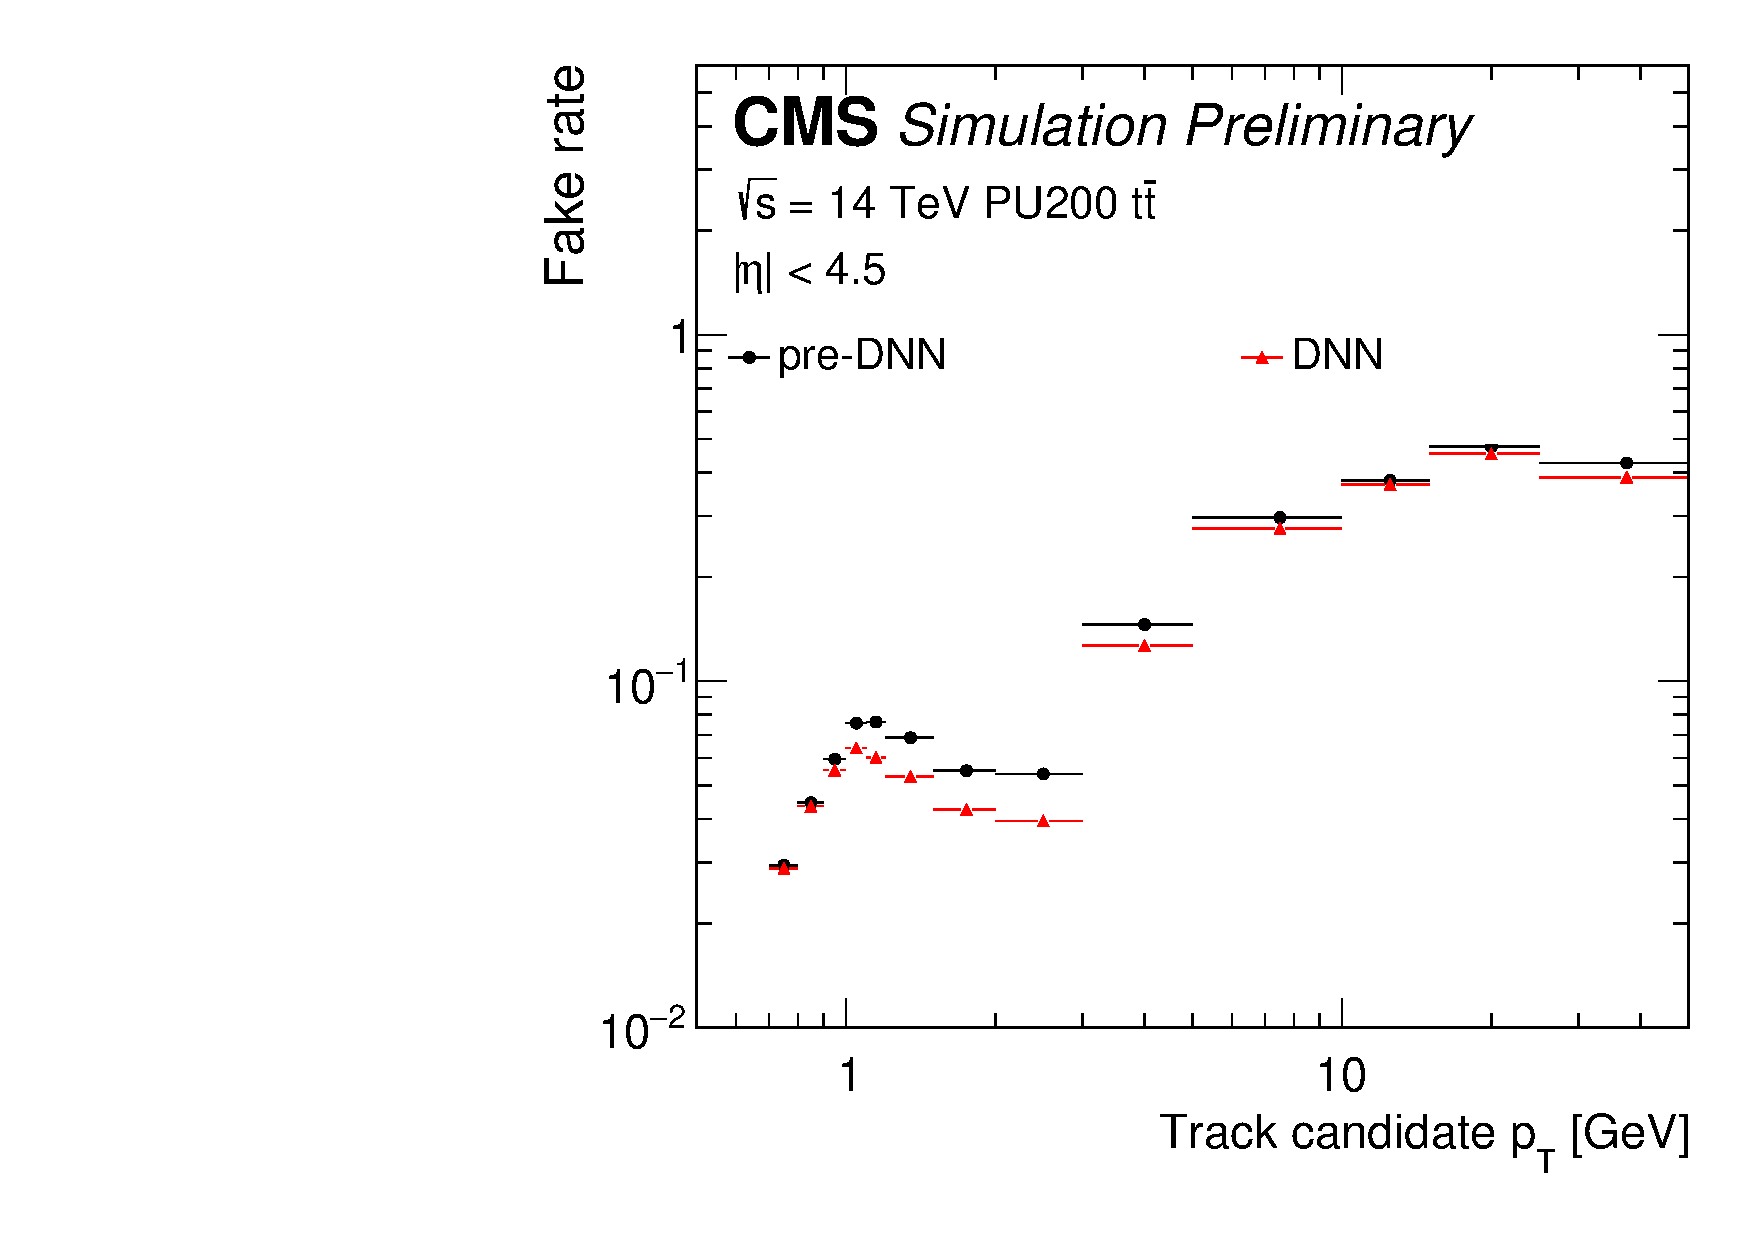
\includegraphics[width=0.45\linewidth]{fig/lst/standalone_DNNvsMaster_pu200_fr_pt_logx_logy.pdf}}
  \qquad
  \subfloat{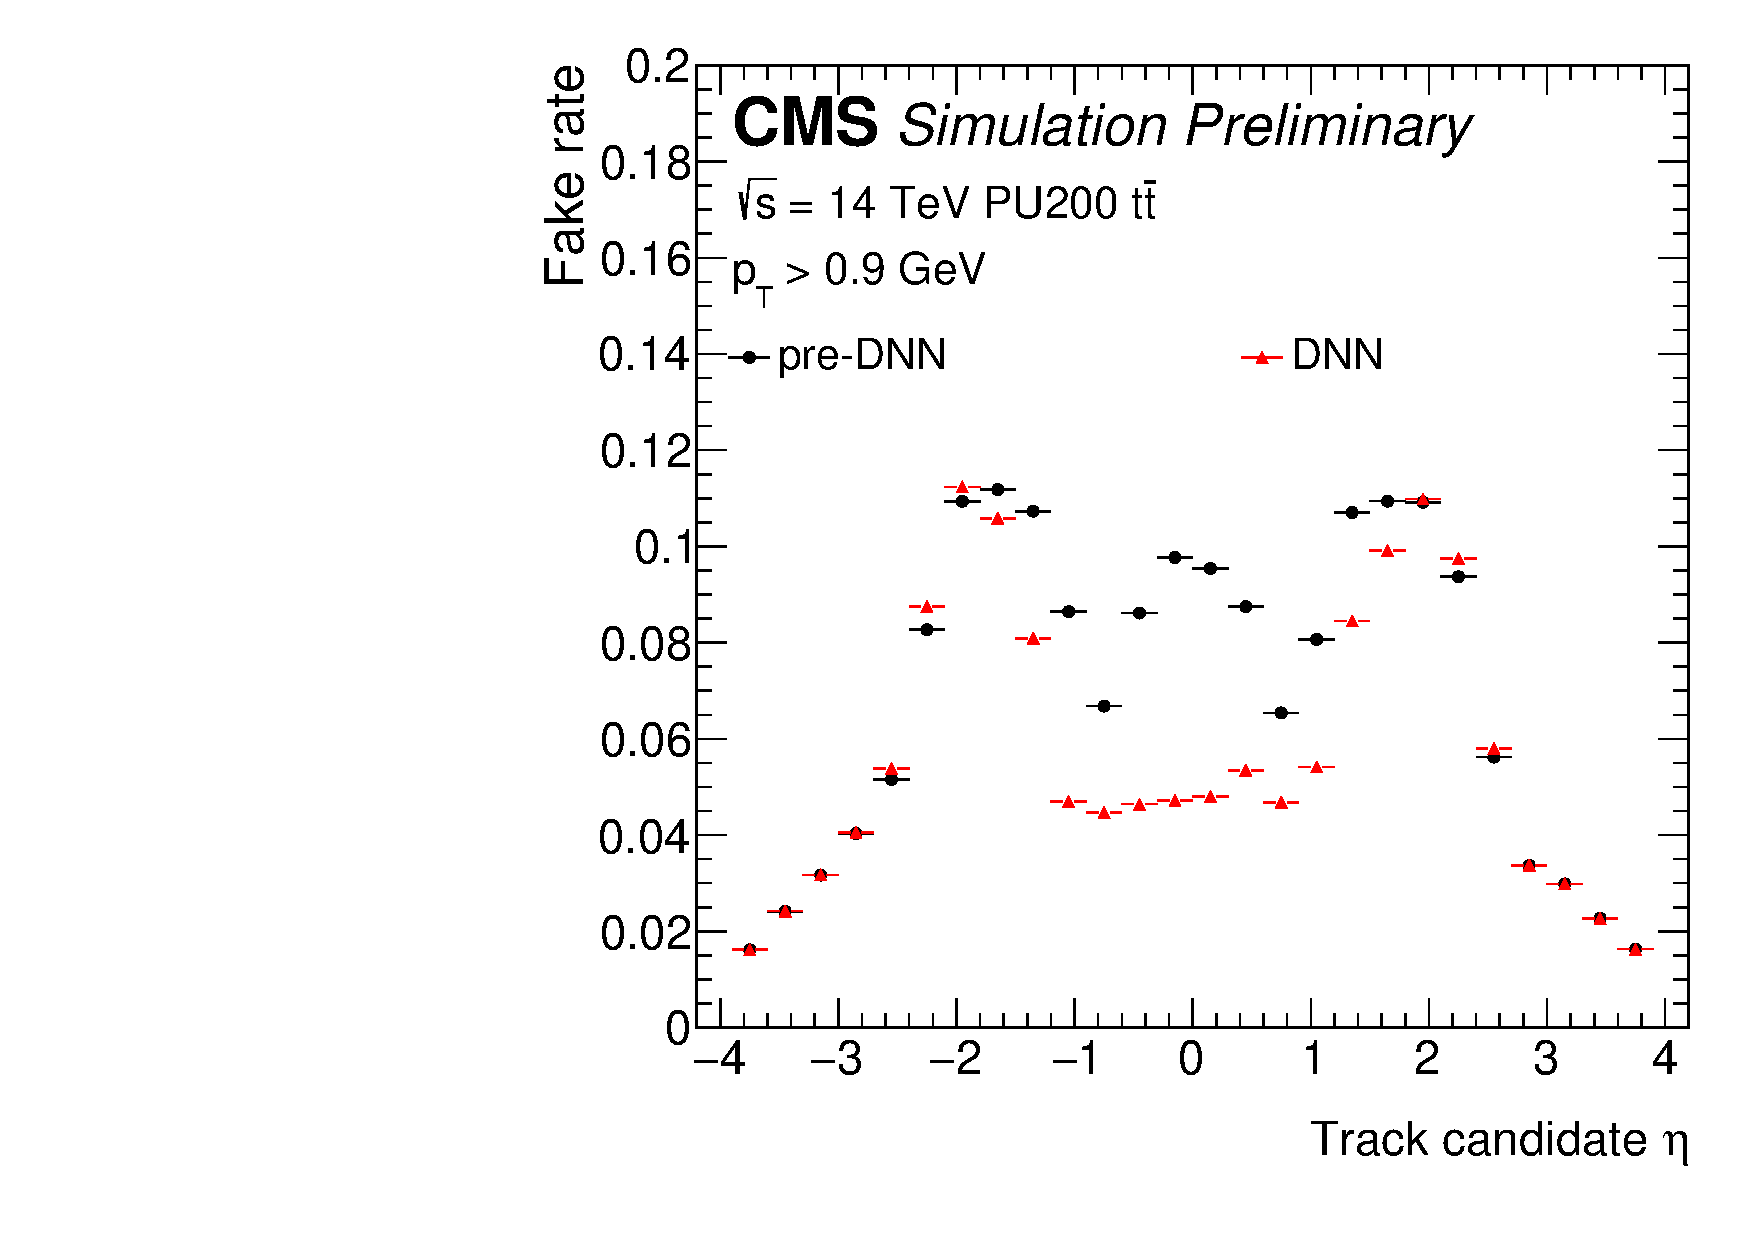
\includegraphics[width=0.45\linewidth]{fig/lst/standalone_DNNvsMaster_pu200_fr_etacourse.pdf}}
  \caption{
      The LST fake rate for all TCs is plotted as a function of \pt (left) and $\eta$ (right).
      Notably, there is a 40\% reduction in the fake rate in the barrel, where the T5 fake rate was previously dominant.
  }
  \label{fig:t5dnn_fkr}
\end{figure}

\begin{figure}[!htb]
  \centering
  \subfloat{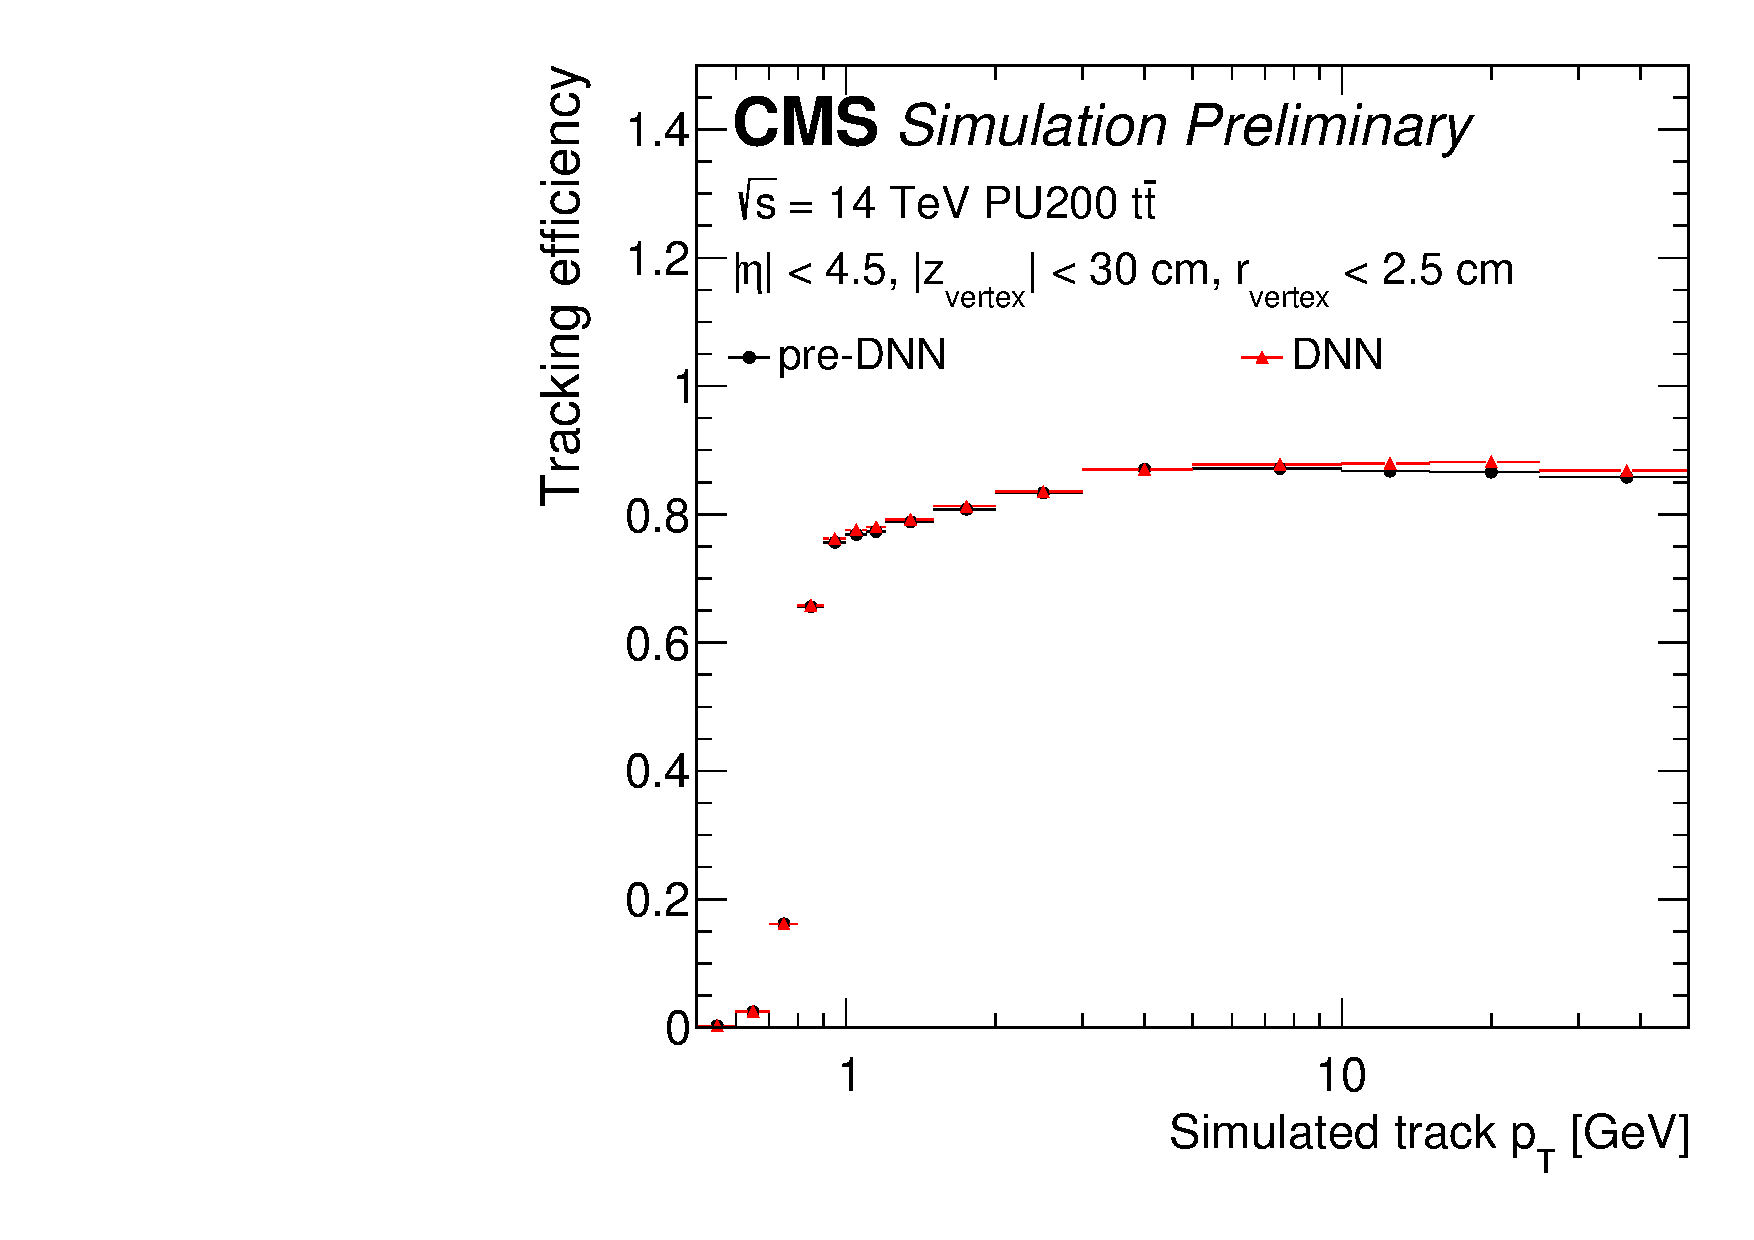
\includegraphics[width=0.45\linewidth]{fig/lst/standalone_DNNvsMaster_pu200_eff_pt_logx.pdf}}
  \qquad
  \subfloat{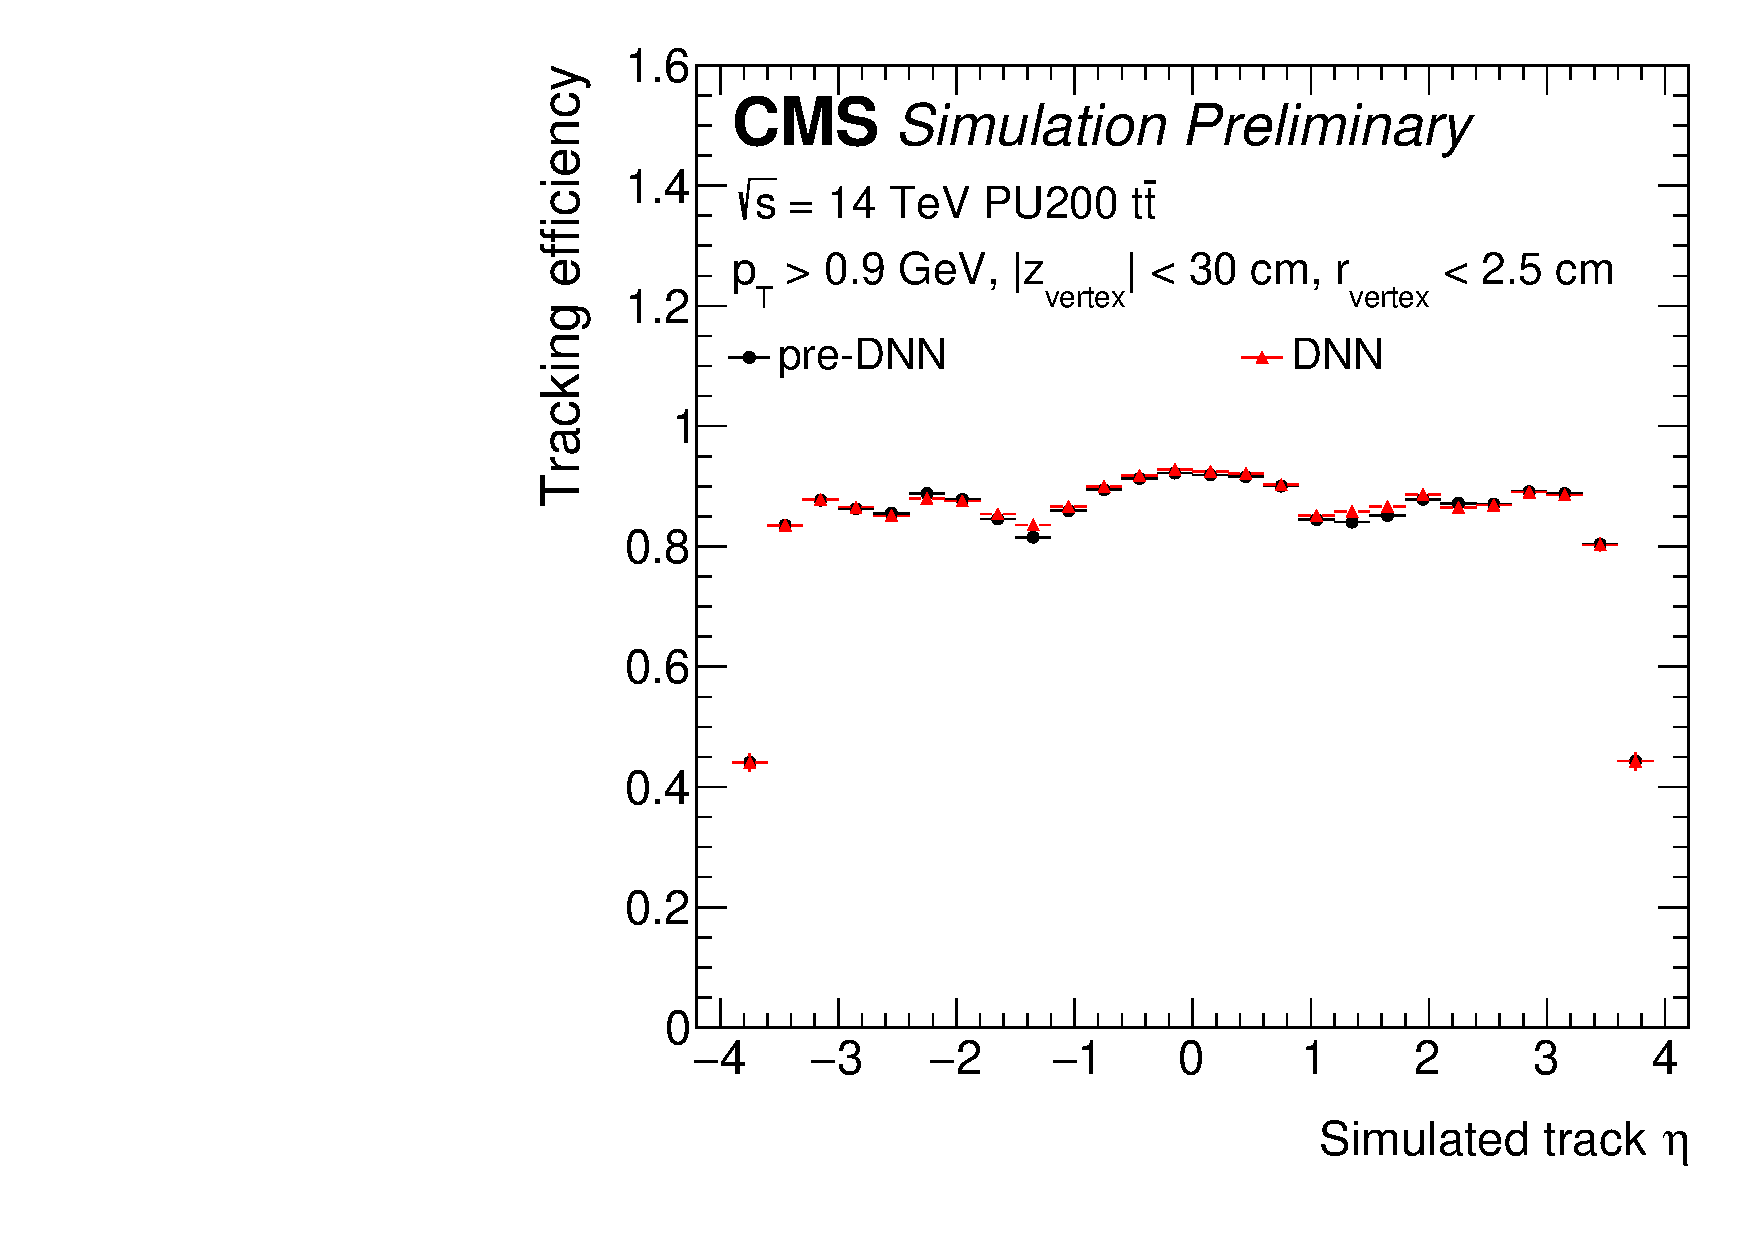
\includegraphics[width=0.45\linewidth]{fig/lst/standalone_DNNvsMaster_pu200_eff_etacourse.pdf}}
  \caption{
      The LST efficiency for all TCs is plotted as a function of \pt (left) and $\eta$ (right).
      The working point for the DNN was selected to match the efficiency of LST, and it is clear that no efficiency is lost.
  }
  \label{fig:t5dnn_eff}
\end{figure}

\begin{figure}[!htb]
  \centering
  \subfloat[]{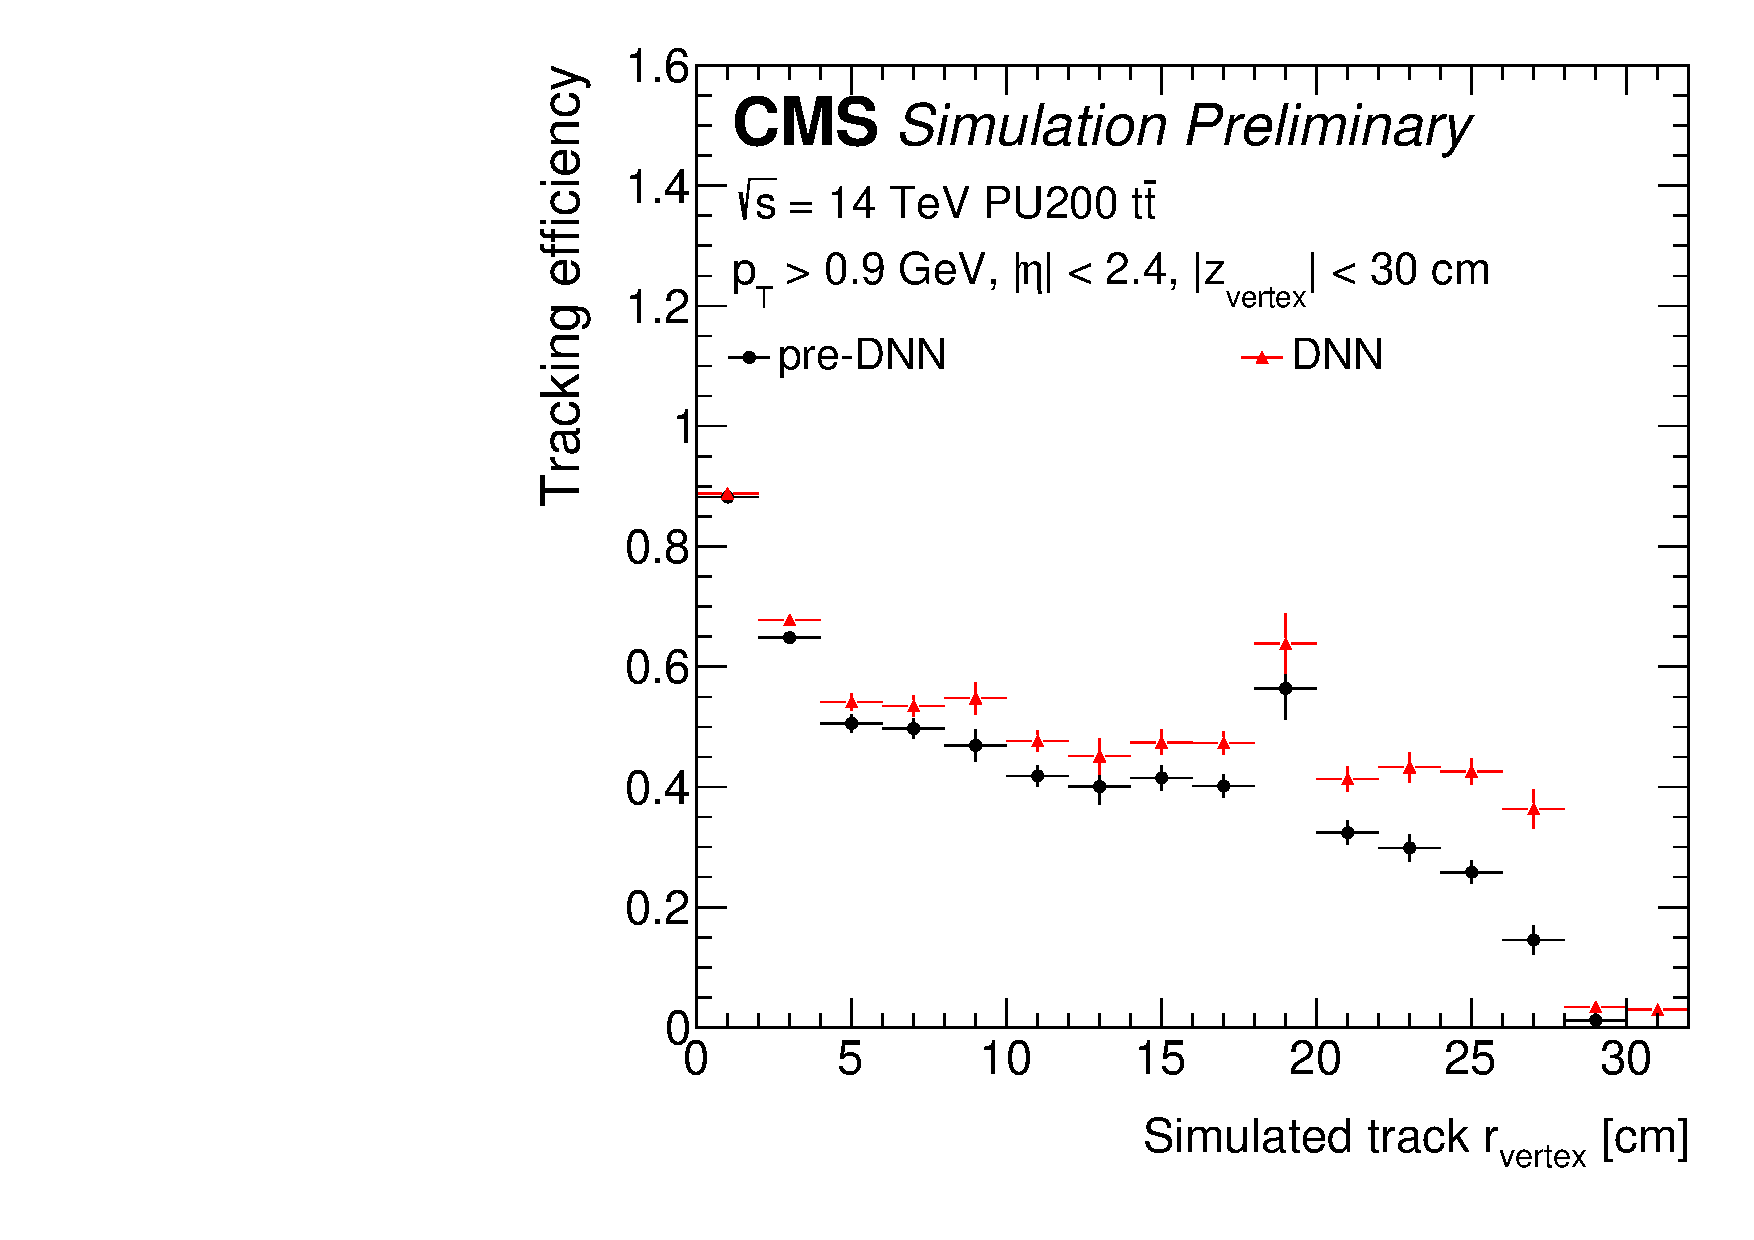
\includegraphics[width=0.45\linewidth]{fig/lst/standalone_DNNvsMaster_pu200_loweta_eff_vxycoarse.pdf}\label{fig:t5dnn_eff_rvertex_ttbar}}
  \qquad
  \subfloat[]{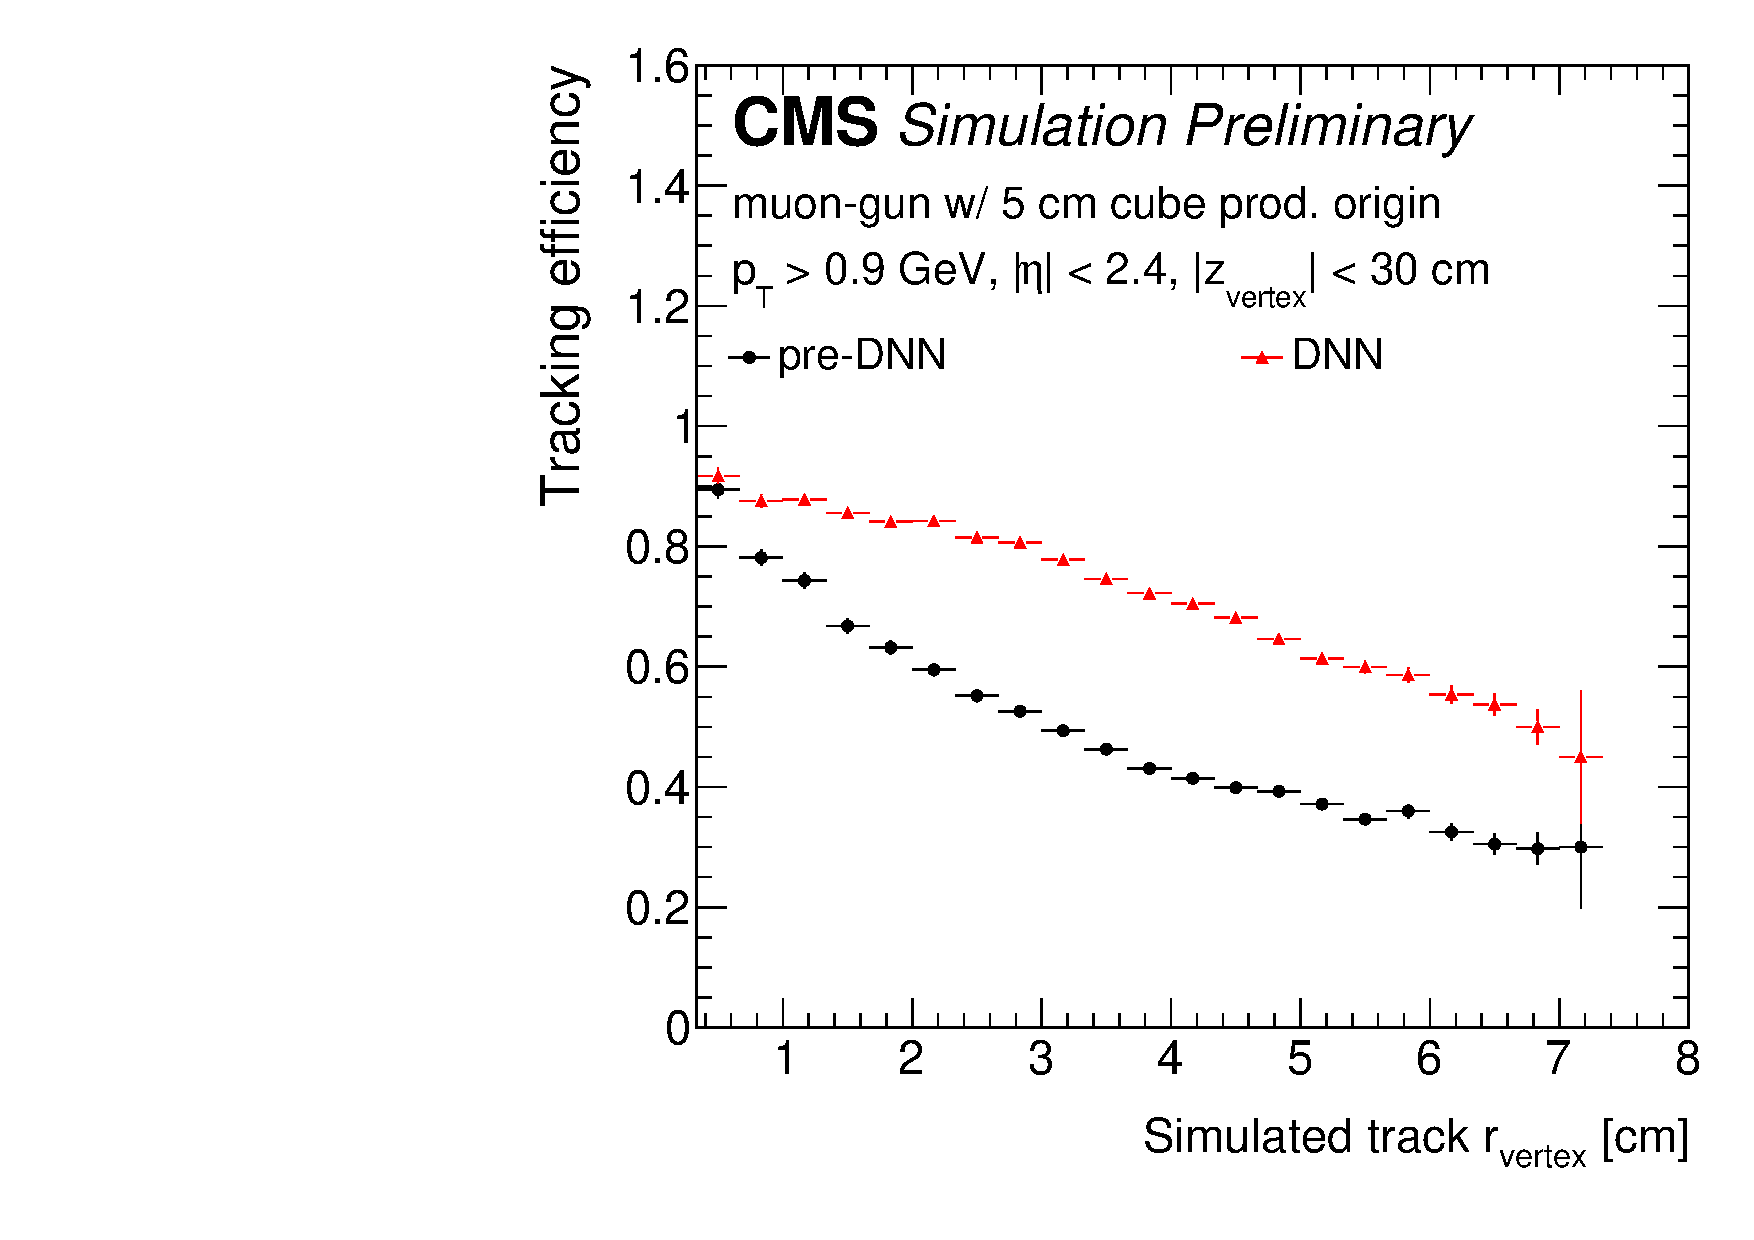
\includegraphics[width=0.45\linewidth]{fig/lst/standalone_DNNvsMaster_cube5_loweta_eff_vxy.pdf}\label{fig:t5dnn_eff_rvertex_cube}}
  \caption{
      The LST efficiency for all TCs is plotted as a function of $r_\text{vertex}$, i.e. the distance to the production vertex measured in the plane transverse to the beamline.
      This plot is made with 1000 \ttbar events with HL-LHC pile-up (a) and 10,000 ``muon-cube'' events where muons are produced at points uniformly distributed across a 5 cm cube (b).
      In both plots, it is clear that the T5-DNN recovers a significant amount of efficiency for displaced tracks.
      In the plot made for \ttbar events, there is a notable peak in the 18 to 20 cm $r_\text{vertex}$ bin.
      This spike in efficiency is due to the detector geometry: there is less detector material in that region, so contributions from material interactions there are lower than in neighboring bins.
  }
\end{figure}

\begin{figure}[!htb]
  \centering
  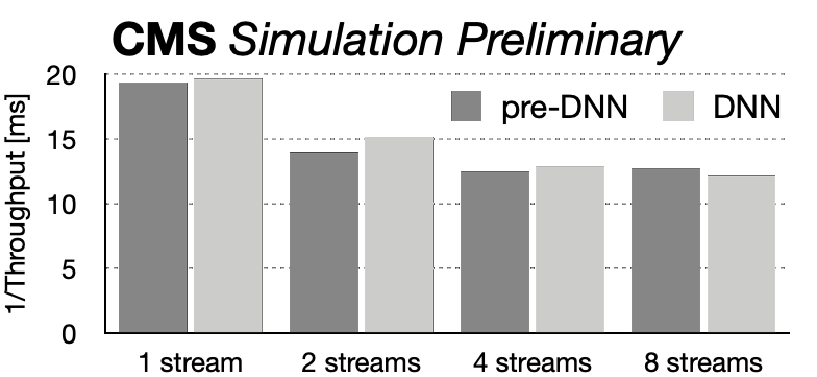
\includegraphics[width=0.85\linewidth]{fig/lst/throughput_vs_streams.pdf}
  \caption{The 2022 CPU usage projections are shown, where it can be seen that R\&D efforts must be undertaken alongside resource increases in order to meet the demand in 2030 when the HL-LHC is planned to start data taking~\cite{CMS-NOTE-2022-008}.}
  \label{fig:streams-vs-throughput}
\end{figure}

\section{Next steps}
